\documentclass[11pt,fleqn, oneside,openany]{book} % Default font size and left-justified equations

% use this list: https://www.educative.io/blog/google-coding-interview

%%%%%%%%%%%%%%%%%%%%%%%%%%%%%%%%%%%%%%%%%%%%
%               Structure
%%%%%%%%%%%%%%%%%%%%%%%%%%%%%%%%%%%%%%%%%%%%
%%%%%%%%%%%%%%%%%%%%%%%%%%%%%%%%%%%%%%%%%
% The Legrand Orange Book
% Structural Definitions File
% Version 2.0 (9/2/15)
%
% Original author:
% Mathias Legrand (legrand.mathias@gmail.com) with modifications by:
% Vel (vel@latextemplates.com)
% 
% This file has been downloaded from:
% http://www.LaTeXTemplates.com
%
% License:
% CC BY-NC-SA 3.0 (http://creativecommons.org/licenses/by-nc-sa/3.0/)
%
%%%%%%%%%%%%%%%%%%%%%%%%%%%%%%%%%%%%%%%%%

%----------------------------------------------------------------------------------------
%	VARIOUS REQUIRED PACKAGES AND CONFIGURATIONS
%----------------------------------------------------------------------------------------

\usepackage[top=3cm,bottom=3cm,left=3cm,right=3cm,headsep=10pt,a4paper]{geometry} % Page margins

\usepackage{graphicx} % Required for including pictures
\graphicspath{{images/}} % Specifies the directory where pictures are stored

\usepackage{lipsum} % Inserts dummy text

\usepackage{tikz} % Required for drawing custom shapes

\usepackage[english]{babel} % English language/hyphenation

\usepackage{enumitem} % Customize lists
\setlist{nolistsep} % Reduce spacing between bullet points and numbered lists

\usepackage{booktabs} % Required for nicer horizontal rules in tables

\usepackage{xcolor} % Required for specifying colors by name
\definecolor{ocre}{RGB}{243,102,25} % Define the orange color used for highlighting throughout the book

%----------------------------------------------------------------------------------------
%	FONTS
%----------------------------------------------------------------------------------------

\usepackage{avant} % Use the Avantgarde font for headings
%\usepackage{times} % Use the Times font for headings
\usepackage{mathptmx} % Use the Adobe Times Roman as the default text font together with math symbols from the Sym­bol, Chancery and Com­puter Modern fonts

\usepackage{microtype} % Slightly tweak font spacing for aesthetics
\usepackage[utf8]{inputenc} % Required for including letters with accents
\usepackage[T1]{fontenc} % Use 8-bit encoding that has 256 glyphs

%----------------------------------------------------------------------------------------
%	BIBLIOGRAPHY AND INDEX
%----------------------------------------------------------------------------------------

\usepackage[citestyle=numeric,sorting=nyt,sortcites=true,autopunct=true,babel=hyphen,hyperref=true,abbreviate=false,backref=true,backend=biber]{biblatex}
\addbibresource{sources/bibliography.bib}
\defbibheading{bibempty}{}

\usepackage{calc} % For simpler calculation - used for spacing the index letter headings correctly
\usepackage{makeidx} % Required to make an index
\makeindex % Tells LaTeX to create the files required for indexing

%----------------------------------------------------------------------------------------
%	MAIN TABLE OF CONTENTS
%----------------------------------------------------------------------------------------

\usepackage{titletoc} % Required for manipulating the table of contents

\contentsmargin{0cm} % Removes the default margin

% Part text styling
\titlecontents{part}[0cm]
{\addvspace{20pt}\centering\large\bfseries}
{}
{}
{}

% Chapter text styling
\titlecontents{chapter}[1.25cm] % Indentation
{\addvspace{12pt}\large\sffamily\bfseries} % Spacing and font options for chapters
{\color{ocre!60}\contentslabel[\Large\thecontentslabel]{1.25cm}\color{ocre}} % Chapter number
{\color{ocre}}  
{\color{ocre!60}\normalsize\;\titlerule*[.5pc]{.}\;\thecontentspage} % Page number

% Section text styling
\titlecontents{section}[1.25cm] % Indentation
{\addvspace{3pt}\sffamily\bfseries} % Spacing and font options for sections
{\contentslabel[\thecontentslabel]{1.25cm}} % Section number
{}
{\hfill\color{black}\thecontentspage} % Page number
[]

% Subsection text styling
\titlecontents{subsection}[1.25cm] % Indentation
{\addvspace{1pt}\sffamily\small} % Spacing and font options for subsections
{\contentslabel[\thecontentslabel]{1.25cm}} % Subsection number
{}
{\ \titlerule*[.5pc]{.}\;\thecontentspage} % Page number
[]

% List of figures
\titlecontents{figure}[0em]
{\addvspace{-5pt}\sffamily}
{\thecontentslabel\hspace*{1em}}
{}
{\ \titlerule*[.5pc]{.}\;\thecontentspage}
[]

% List of tables
\titlecontents{table}[0em]
{\addvspace{-5pt}\sffamily}
{\thecontentslabel\hspace*{1em}}
{}
{\ \titlerule*[.5pc]{.}\;\thecontentspage}
[]

%----------------------------------------------------------------------------------------
%	MINI TABLE OF CONTENTS IN PART HEADS
%----------------------------------------------------------------------------------------

% Chapter text styling
\titlecontents{lchapter}[0em] % Indenting
{\addvspace{15pt}\large\sffamily\bfseries} % Spacing and font options for chapters
{\color{ocre}\contentslabel[\Large\thecontentslabel]{1.25cm}\color{ocre}} % Chapter number
{}  
{\color{ocre}\normalsize\sffamily\bfseries\;\titlerule*[.5pc]{.}\;\thecontentspage} % Page number

% Section text styling
\titlecontents{lsection}[0em] % Indenting
{\sffamily\small} % Spacing and font options for sections
{\contentslabel[\thecontentslabel]{1.25cm}} % Section number
{}
{}

% Subsection text styling
\titlecontents{lsubsection}[.5em] % Indentation
{\normalfont\footnotesize\sffamily} % Font settings
{}
{}
{}

%----------------------------------------------------------------------------------------
%	PAGE HEADERS
%----------------------------------------------------------------------------------------

\usepackage{fancyhdr} % Required for header and footer configuration

\pagestyle{fancy}
\renewcommand{\chaptermark}[1]{\markboth{\sffamily\normalsize\bfseries\chaptername\ \thechapter.\ #1}{}} % Chapter text font settings
\renewcommand{\sectionmark}[1]{\markright{\sffamily\normalsize\thesection\hspace{5pt}#1}{}} % Section text font settings
\fancyhf{} \fancyhead[LE,RO]{\sffamily\normalsize\thepage} % Font setting for the page number in the header
\fancyhead[LO]{\rightmark} % Print the nearest section name on the left side of odd pages
\fancyhead[RE]{\leftmark} % Print the current chapter name on the right side of even pages
\renewcommand{\headrulewidth}{0.5pt} % Width of the rule under the header
\addtolength{\headheight}{2.5pt} % Increase the spacing around the header slightly
\renewcommand{\footrulewidth}{0pt} % Removes the rule in the footer
\fancypagestyle{plain}{\fancyhead{}\renewcommand{\headrulewidth}{0pt}} % Style for when a plain pagestyle is specified

% Removes the header from odd empty pages at the end of chapters
\makeatletter
\renewcommand{\cleardoublepage}{
\clearpage\ifodd\c@page\else
\hbox{}
\vspace*{\fill}
\thispagestyle{empty}
\newpage
\fi}

%----------------------------------------------------------------------------------------
%	THEOREM STYLES
%----------------------------------------------------------------------------------------


\usepackage{amsmath,amsfonts,amssymb,amsthm,mathtools} % For math equations, theorems, symbols, etc
\DeclarePairedDelimiter\ceil{\lceil}{\rceil}
\DeclarePairedDelimiter\floor{\lfloor}{\rfloor}

\newcommand{\intoo}[2]{\mathopen{]}#1\,;#2\mathclose{[}}
\newcommand{\ud}{\mathop{\mathrm{{}d}}\mathopen{}}
\newcommand{\intff}[2]{\mathopen{[}#1\,;#2\mathclose{]}}
\newtheorem{notation}{Notation}[chapter]

% Boxed/framed environments
\newtheoremstyle{ocrenumbox}% % Theorem style name
{0pt}% Space above
{0pt}% Space below
{\normalfont}% % Body font
{}% Indent amount
{\small\bf\sffamily\color{ocre}}% % Theorem head font
{\;}% Punctuation after theorem head
{0.25em}% Space after theorem head
{\small\sffamily\color{ocre}\thmname{#1}\nobreakspace\thmnumber{\@ifnotempty{#1}{}\@upn{#2}}% Theorem text (e.g. Theorem 2.1)
\thmnote{\nobreakspace\the\thm@notefont\sffamily\bfseries\color{black}---\nobreakspace#3.}} % Optional theorem note
\renewcommand{\qedsymbol}{$\blacksquare$}% Optional qed square

\newtheoremstyle{blacknumex}% Theorem style name
{5pt}% Space above
{5pt}% Space below
{\normalfont}% Body font
{} % Indent amount
{\small\bf\sffamily}% Theorem head font
{\;}% Punctuation after theorem head
{0.25em}% Space after theorem head
{\small\sffamily{\tiny\ensuremath{\blacksquare}}\nobreakspace\thmname{#1}\nobreakspace\thmnumber{\@ifnotempty{#1}{}\@upn{#2}}% Theorem text (e.g. Theorem 2.1)
\thmnote{\nobreakspace\the\thm@notefont\sffamily\bfseries---\nobreakspace#3.}}% Optional theorem note

\newtheoremstyle{blacknumbox} % Theorem style name
{0pt}% Space above
{0pt}% Space below
{\normalfont}% Body font
{}% Indent amount
{\small\bf\sffamily}% Theorem head font
{\;}% Punctuation after theorem head
{0.25em}% Space after theorem head
{\small\sffamily\thmname{#1}\nobreakspace\thmnumber{\@ifnotempty{#1}{}\@upn{#2}}% Theorem text (e.g. Theorem 2.1)
\thmnote{\nobreakspace\the\thm@notefont\sffamily\bfseries---\nobreakspace#3.}}% Optional theorem note

% Non-boxed/non-framed environments
\newtheoremstyle{ocrenum}% % Theorem style name
{5pt}% Space above
{5pt}% Space below
{\normalfont}% % Body font
{}% Indent amount
{\small\bf\sffamily\color{ocre}}% % Theorem head font
{\;}% Punctuation after theorem head
{0.25em}% Space after theorem head
{\small\sffamily\color{ocre}\thmname{#1}\nobreakspace\thmnumber{\@ifnotempty{#1}{}\@upn{#2}}% Theorem text (e.g. Theorem 2.1)
\thmnote{\nobreakspace\the\thm@notefont\sffamily\bfseries\color{black}---\nobreakspace#3.}} % Optional theorem note
\renewcommand{\qedsymbol}{$\blacksquare$}% Optional qed square
\makeatother

% Defines the theorem text style for each type of theorem to one of the three styles above
\newcounter{dummy} 
\numberwithin{dummy}{section}
\theoremstyle{ocrenumbox}
\newtheorem{theoremeT}[dummy]{Theorem}

\newtheorem{problem}{Exercise}[chapter]
\newtheorem{exerciseT}{Problem}
\theoremstyle{blacknumex}
\newtheorem{solution}{Solution}[chapter]
\newtheorem{solutionT}{solution}[chapter]
\theoremstyle{blacknumex}
\newtheorem{exampleT}{Example}[chapter]
\theoremstyle{blacknumbox}
\newtheorem{vocabulary}{Vocabulary}[chapter]
\newtheorem{definitionT}{Definition}[section]
\newtheorem{corollaryT}[dummy]{Corollary}
\theoremstyle{ocrenum}
\newtheorem{proposition}[dummy]{Proposition}

%----------------------------------------------------------------------------------------
%	DEFINITION OF COLORED BOXES
%----------------------------------------------------------------------------------------

\RequirePackage[framemethod=default]{mdframed} % Required for creating the theorem, definition, exercise and corollary boxes

% Theorem box
\newmdenv[skipabove=7pt,
skipbelow=7pt,
backgroundcolor=black!5,
linecolor=ocre,
innerleftmargin=5pt,
innerrightmargin=5pt,
innertopmargin=5pt,
leftmargin=0cm,
rightmargin=0cm,
innerbottommargin=5pt]{tBox}

% Exercise box	  
\newmdenv[skipabove=7pt,
skipbelow=7pt,
rightline=false,
leftline=true,
topline=false,
bottomline=false,
backgroundcolor=ocre!10,
linecolor=ocre,
innerleftmargin=5pt,
innerrightmargin=5pt,
innertopmargin=5pt,
innerbottommargin=5pt,
leftmargin=0cm,
rightmargin=0cm,
linewidth=4pt]{eBox}	

% Definition box
\newmdenv[skipabove=7pt,
skipbelow=7pt,
rightline=false,
leftline=true,
topline=false,
bottomline=false,
linecolor=ocre,
innerleftmargin=5pt,
innerrightmargin=5pt,
innertopmargin=0pt,
leftmargin=0cm,
rightmargin=0cm,
linewidth=4pt,
innerbottommargin=0pt]{dBox}	

% Corollary box
\newmdenv[skipabove=7pt,
skipbelow=7pt,
rightline=false,
leftline=true,
topline=false,
bottomline=false,
linecolor=gray,
backgroundcolor=black!5,
innerleftmargin=5pt,
innerrightmargin=5pt,
innertopmargin=5pt,
leftmargin=0cm,
rightmargin=0cm,
linewidth=4pt,
innerbottommargin=5pt]{cBox}

% Creates an environment for each type of theorem and assigns it a theorem text style from the "Theorem Styles" section above and a colored box from above
\newenvironment{theorem}{\begin{tBox}\begin{theoremeT}}{\end{theoremeT}\end{tBox}}
\newenvironment{exercise}{\begin{eBox}\begin{exerciseT}}{\hfill{\color{ocre}\tiny\ensuremath{\blacksquare}}\end{exerciseT}\end{eBox}}				  
\newenvironment{definition}{\begin{dBox}\begin{definitionT}}{\end{definitionT}\end{dBox}}	
\newenvironment{example}{\begin{exampleT}}{\hfill{\tiny\ensuremath{\blacksquare}}\end{exampleT}}		
\newenvironment{corollary}{\begin{cBox}\begin{corollaryT}}{\end{corollaryT}\end{cBox}}	

%----------------------------------------------------------------------------------------
%	REMARK ENVIRONMENT
%----------------------------------------------------------------------------------------

\newenvironment{remark}{\par\vspace{10pt}\small % Vertical white space above the remark and smaller font size
\begin{list}{}{
\leftmargin=35pt % Indentation on the left
\rightmargin=25pt}\item\ignorespaces % Indentation on the right
\makebox[-2.5pt]{\begin{tikzpicture}[overlay]
\node[draw=ocre!60,line width=1pt,circle,fill=ocre!25,font=\sffamily\bfseries,inner sep=2pt,outer sep=0pt] at (-15pt,0pt){\textcolor{ocre}{R}};\end{tikzpicture}} % Orange R in a circle
\advance\baselineskip -1pt}{\end{list}\vskip5pt} % Tighter line spacing and white space after remark

%----------------------------------------------------------------------------------------
%	SECTION NUMBERING IN THE MARGIN
%----------------------------------------------------------------------------------------

\makeatletter
\renewcommand{\@seccntformat}[1]{\llap{\textcolor{ocre}{\csname the#1\endcsname}\hspace{1em}}}                    
\renewcommand{\section}{\@startsection{section}{1}{\z@}
{-4ex \@plus -1ex \@minus -.4ex}
{1ex \@plus.2ex }
{\normalfont\large\sffamily\bfseries}}
\renewcommand{\subsection}{\@startsection {subsection}{2}{\z@}
{-3ex \@plus -0.1ex \@minus -.4ex}
{0.5ex \@plus.2ex }
{\normalfont\sffamily\bfseries}}
\renewcommand{\subsubsection}{\@startsection {subsubsection}{3}{\z@}
{-2ex \@plus -0.1ex \@minus -.2ex}
{.2ex \@plus.2ex }
{\normalfont\small\sffamily\bfseries}}                        
\renewcommand\paragraph{\@startsection{paragraph}{4}{\z@}
{-2ex \@plus-.2ex \@minus .2ex}
{.1ex}
{\normalfont\small\sffamily\bfseries}}

%----------------------------------------------------------------------------------------
%	PART HEADINGS
%----------------------------------------------------------------------------------------

% numbered part in the table of contents
\newcommand{\@mypartnumtocformat}[2]{%
\setlength\fboxsep{0pt}%
\noindent\colorbox{ocre!20}{\strut\parbox[c][.7cm]{\ecart}{\color{ocre!70}\Large\sffamily\bfseries\centering#1}}\hskip\esp\colorbox{ocre!40}{\strut\parbox[c][.7cm]{\linewidth-\ecart-\esp}{\Large\sffamily\centering#2}}}%
%%%%%%%%%%%%%%%%%%%%%%%%%%%%%%%%%%
% unnumbered part in the table of contents
\newcommand{\@myparttocformat}[1]{%
\setlength\fboxsep{0pt}%
\noindent\colorbox{ocre!40}{\strut\parbox[c][.7cm]{\linewidth}{\Large\sffamily\centering#1}}}%
%%%%%%%%%%%%%%%%%%%%%%%%%%%%%%%%%%
\newlength\esp
\setlength\esp{4pt}
\newlength\ecart
\setlength\ecart{1.2cm-\esp}
\newcommand{\thepartimage}{}%
\newcommand{\partimage}[1]{\renewcommand{\thepartimage}{#1}}%
\def\@part[#1]#2{%
\ifnum \c@secnumdepth >-2\relax%
\refstepcounter{part}%
\addcontentsline{toc}{part}{\texorpdfstring{\protect\@mypartnumtocformat{\thepart}{#1}}{\partname~\thepart\ ---\ #1}}
\else%
\addcontentsline{toc}{part}{\texorpdfstring{\protect\@myparttocformat{#1}}{#1}}%
\fi%
\startcontents%
\markboth{}{}%
{\thispagestyle{empty}%
\begin{tikzpicture}[remember picture,overlay]%
\node at (current page.north west){\begin{tikzpicture}[remember picture,overlay]%	
\fill[ocre!20](0cm,0cm) rectangle (\paperwidth,-\paperheight);
\node[anchor=north] at (4cm,-3.25cm){\color{ocre!40}\fontsize{220}{100}\sffamily\bfseries\@Roman\c@part}; 
\node[anchor=south east] at (\paperwidth-1cm,-\paperheight+1cm){\parbox[t][][t]{8.5cm}{
\printcontents{l}{0}{\setcounter{tocdepth}{1}}%
}};
\node[anchor=north east] at (\paperwidth-1.5cm,-3.25cm){\parbox[t][][t]{15cm}{\strut\raggedleft\color{white}\fontsize{30}{30}\sffamily\bfseries#2}};
\end{tikzpicture}};
\end{tikzpicture}}%
\@endpart}
\def\@spart#1{%
\startcontents%
\phantomsection
{\thispagestyle{empty}%
\begin{tikzpicture}[remember picture,overlay]%
\node at (current page.north west){\begin{tikzpicture}[remember picture,overlay]%	
\fill[ocre!20](0cm,0cm) rectangle (\paperwidth,-\paperheight);
\node[anchor=north east] at (\paperwidth-1.5cm,-3.25cm){\parbox[t][][t]{15cm}{\strut\raggedleft\color{white}\fontsize{30}{30}\sffamily\bfseries#1}};
\end{tikzpicture}};
\end{tikzpicture}}
\addcontentsline{toc}{part}{\texorpdfstring{%
\setlength\fboxsep{0pt}%
\noindent\protect\colorbox{ocre!40}{\strut\protect\parbox[c][.7cm]{\linewidth}{\Large\sffamily\protect\centering #1\quad\mbox{}}}}{#1}}%
\@endpart}
\def\@endpart{\vfil\newpage
\if@twoside
\if@openright
\null
\thispagestyle{empty}%
\newpage
\fi
\fi
\if@tempswa
\twocolumn
\fi}

%----------------------------------------------------------------------------------------
%	CHAPTER HEADINGS
%----------------------------------------------------------------------------------------

% A switch to conditionally include a picture, implemented by  Christian Hupfer
\newif\ifusechapterimage
\usechapterimagetrue
\newcommand{\thechapterimage}{}%
\newcommand{\chapterimage}[1]{\ifusechapterimage\renewcommand{\thechapterimage}{#1}\fi}%
\def\@makechapterhead#1{%
{\parindent \z@ \raggedright \normalfont
\ifnum \c@secnumdepth >\m@ne
\if@mainmatter
\begin{tikzpicture}[remember picture,overlay]
\node at (current page.north west)
{\begin{tikzpicture}[remember picture,overlay]
\node[anchor=north west,inner sep=0pt] at (0,0) {\ifusechapterimage\includegraphics[width=\paperwidth]{\thechapterimage}\fi};
\draw[anchor=west] (\Gm@lmargin,-4cm) node [line width=2pt,rounded corners=15pt,draw=ocre,fill=white,fill opacity=0.5,inner sep=15pt]{\strut\makebox[22cm]{}};
\draw[anchor=west] (\Gm@lmargin+.3cm,-4cm) node {\huge\sffamily\bfseries\color{black}\thechapter. #1\strut};
\end{tikzpicture}};
\end{tikzpicture}
\else
\begin{tikzpicture}[remember picture,overlay]
\node at (current page.north west)
{\begin{tikzpicture}[remember picture,overlay]
\node[anchor=north west,inner sep=0pt] at (0,0) {\ifusechapterimage\includegraphics[width=\paperwidth]{\thechapterimage}\fi};
\draw[anchor=west] (\Gm@lmargin,-4cm) node [line width=2pt,rounded corners=15pt,draw=ocre,fill=white,fill opacity=0.5,inner sep=15pt]{\strut\makebox[22cm]{}};
\draw[anchor=west] (\Gm@lmargin+.3cm,-4cm) node {\huge\sffamily\bfseries\color{black}#1\strut};
\end{tikzpicture}};
\end{tikzpicture}
\fi\fi\par\vspace*{100\p@}}}

%-------------------------------------------

\def\@makeschapterhead#1{%
\begin{tikzpicture}[remember picture,overlay]
\node at (current page.north west)
{\begin{tikzpicture}[remember picture,overlay]
\node[anchor=north west,inner sep=0pt] at (0,0) {\ifusechapterimage\includegraphics[width=\paperwidth]{\thechapterimage}\fi};
\draw[anchor=west] (\Gm@lmargin,-4cm) node [line width=2pt,rounded corners=15pt,draw=ocre,fill=white,fill opacity=0.5,inner sep=15pt]{\strut\makebox[22cm]{}};
\draw[anchor=west] (\Gm@lmargin+.3cm,-4cm) node {\huge\sffamily\bfseries\color{black}#1\strut};
\end{tikzpicture}};
\end{tikzpicture}
\par\vspace*{100\p@}}
\makeatother

%----------------------------------------------------------------------------------------
%	HYPERLINKS IN THE DOCUMENTS
%----------------------------------------------------------------------------------------

\usepackage{hyperref}
\hypersetup{hidelinks,backref=true,pagebackref=true,hyperindex=true,colorlinks=false,breaklinks=true,urlcolor= ocre,bookmarks=true,bookmarksopen=false,pdftitle={Title},pdfauthor={Author}}
\usepackage{bookmark}
\bookmarksetup{
open,
numbered,
addtohook={%
\ifnum\bookmarkget{level}=0 % chapter
\bookmarksetup{bold}%
\fi
\ifnum\bookmarkget{level}=-1 % part
\bookmarksetup{color=ocre,bold}%
\fi
}
}

%----------------------------------------------------------------------------------------
%	LISTINGS
%----------------------------------------------------------------------------------------
%----------------------------------------------------------------------------------------
%	LISTINGS
%----------------------------------------------------------------------------------------
\usepackage{listings}
\lstset{language=C++}
\lstset{
	basicstyle=\footnotesize\ttfamily,
	breaklines=true,
	showstringspaces=false,
	numbers=left,
	backgroundcolor=\color{bgcolor},
	commentstyle=\color{gray},
	keywordstyle=\color{blue},
	keywordstyle=[2]\color{teal},   % cyan or teal can also be a good choice, use \bfseries for bold
	frame=none,                     % adds a frame around the code
	tabsize=2,                      % sets default tabsize to 2 spaces
	captionpos=b,                   % sets the caption-position to bottom
	morekeywords=[2]{}              % if you want to add more keywords to the set
	__
}

\definecolor{mygreen}{RGB}{28,172,0} % color values Red, Green, Blue
\definecolor{mylilas}{RGB}{170,55,241}
\lstset{language=Matlab,%
    %basicstyle=\color{red},
    breaklines=true,%
    morekeywords={matlab2tikz},
    keywordstyle=\color{blue},%
    morekeywords=[2]{1}, keywordstyle=[2]{\color{black}},
    identifierstyle=\color{black},%
    stringstyle=\color{mylilas},
    commentstyle=\color{mygreen},%
    showstringspaces=false,%without this there will be a symbol in the places where there is a space
    numbers=left,%
    numberstyle={\tiny \color{black}},% size of the numbers
    numbersep=9pt, % this defines how far the numbers are from the text
    emph=[1]{for,end,break},emphstyle=[1]\color{red}, %some words to emphasise
    %emph=[2]{word1,word2}, emphstyle=[2]{style},    
}

\usepackage{color}
\definecolor{bgcolor}{rgb}{0.98,0.98,0.98}


%----------------------------------------------------------------------------------------

%	QandA

%----------------------------------------------------------------------------------------

\newenvironment{QandA}{\begin{enumerate}[label=\bfseries Q.\arabic*.,leftmargin=2em,rightmargin=2em]\bfseries}{\end{enumerate}}
\newenvironment{answered}{\par\normalfont}{}
%----------------------------------------------------------------------------------------
%	ALGORITHM
%----------------------------------------------------------------------------------------
\usepackage[]{algorithm2e}

\RestyleAlgo{boxruled}
\usepackage{mdframed,framed}

\SetKwProg{Fn}{Function}{}{}
\SetKwRepeat{Do}{do}{while}%
\SetKwFunction{CreateHashSet}{CreateHashSet<int>}


\DeclarePairedDelimiter\abs{\lvert}{\rvert}%
\DeclarePairedDelimiter\norm{\lVert}{\rVert}%

% Swap the definition of \abs* and \norm*, so that \abs
% and \norm resizes the size of the brackets, and the 
% starred version does not.
\makeatletter
\let\oldabs\abs
\def\abs{\@ifstar{\oldabs}{\oldabs*}}
%
\let\oldnorm\norm
\def\norm{\@ifstar{\oldnorm}{\oldnorm*}}
\makeatother

\usepackage[makeroom]{cancel}



\interfootnotelinepenalty=10000

\begin{document}

%\frontmatter
%\begingroup
%\thispagestyle{empty}
%\begin{tikzpicture}[remember picture,overlay]
%  \coordinate [below=12cm] (midpoint) at (current page.north);
%  \node at (current page.north west)
%  {\begin{tikzpicture}[remember picture,overlay]
%      \node[anchor=north west,inner sep=0pt] at (0,0) {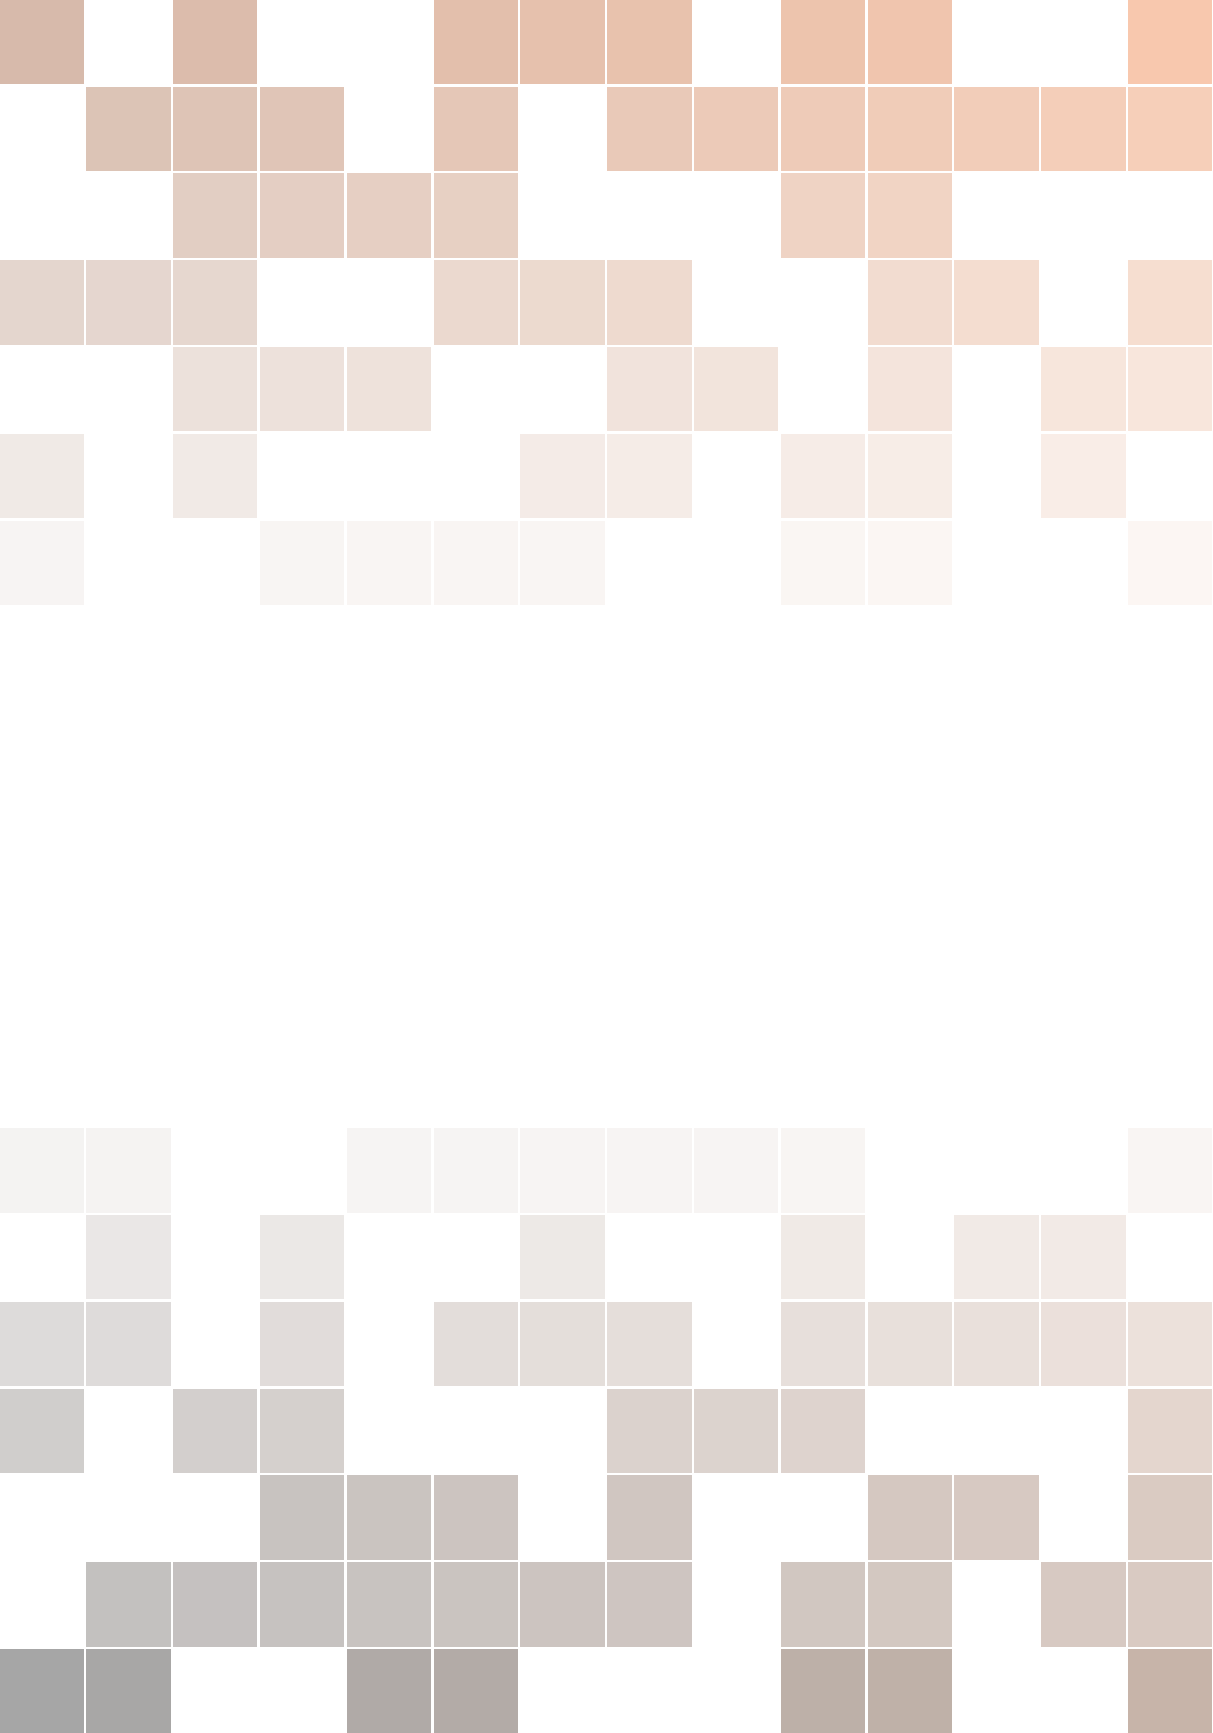
\includegraphics[width=\paperwidth]{images/background}}; % Background image
%\textsl{}
%      \draw[anchor=north] (midpoint) node [fill=ocre!30!white,fill opacity=0.6,text opacity=1,inner sep=1cm]{\Huge\centering\bfseries\sffamily\parbox[c][][t]{\paperwidth}{\centering Coding Interview Essentials\\[15pt] % Book title
%      {\Large - }\\[20pt] % Subtitle
%      {\huge Davide Spataro}}}; % Author name
%    \end{tikzpicture}};
%\end{tikzpicture}
%\vfill
%\endgroup


\includepdf[pages={2},fitpaper=true]{images/book_covers1.pdf}


\usechapterimagefalse % If you don't want to include a chapter image, use this to toggle images off - it can be enabled later with \usechapterimagetrue

%\chapterimage{images/header} % Table of contents heading image

\pagestyle{empty} % No headers

\tableofcontents % Print the table of contents itself

%\lstlistoflistings
%\listoffigures
%\listoftables

%\cleardoublepage % Forces the first chapter to start on an odd page so it's on the right

%pagestyle{fancy} % Print headers again
	
%!TEX root = ../main.tex
%%%%%%%%%%%%%%%%%%%%%%%%%%%%%%%%%%
% Links:
%
% Difficulty: Companies: 
%%%%%%%%%%%%%%%%%%%%%%%%%%%%%%%%%%


%\begin{figure} \centering 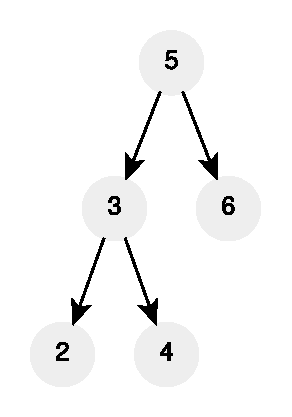
\includegraphics[width=\textwidth]{sources/max_manhattan/images/example1}
%   \caption[Sample short cpation]{Sample Caption}. \label{fig:max_manhattan:example1} \end{figure}

\chapter{Max in manhattan neighborhood$^{K}$}
\label{ch:max_manhattan}

\section*{Introduction}

This chapter discusses a very interesting problem based on the concept of the
\textit{Manhattan distance} \footnote{Also known as \textit{taxicab distance}.}; an alternative way to measure distances that is particularly useful in real life. Imagine
you need to measure the distance between two points on a map. You can use the  Euclidean
distance and come up with a number that in reality is not going to be super helpful unless you can fly. This is because that number is not going to tell you the actual distance you need to
cover if you want to get to your destination by moving on land. For example, what is the distance
between the Empire State building and Times Square in New York? If you are not naturally equipped
with wings then what you actually do is to jump in a car or a cab or a bike and follow the grid pattern of
streets of Manhattan. This means that you would probably have to cover around 15 blocks north and 3 south (See
Figure \ref{fig:max_manhattan:distance_manhattan}). The idea of measuring the distance by
counting the number of steps we take in the north-south or west-east directions underlies what is
known as the taxicab distance. In this framework, the distance is not represented as a straight line
going from point A to point B (like it would for the Euclidean distance) but it is a zig-zagged
sequence of vertical and horizontal segments, representing movements along the north-south and
east-west axis. Therefore, the formula for measuring the taxicab distance is all about measuring
the length of the horizontal and vertical segments. The formula for measuring the Manhattan distance in
Equation \ref{eq:max_manhattan:distance_formula} .
\begin{equation}
    d = |x_1-x_2|+|y_1-y_2|
    \label{eq:max_manhattan:distance_formula}
\end{equation}

The problem in this chapter will challenge you to find, for each cell of a given matrix, the largest
value in any cell sitting at a Manahtann distance below a certain threshold.

\begin{figure}
    \centering
    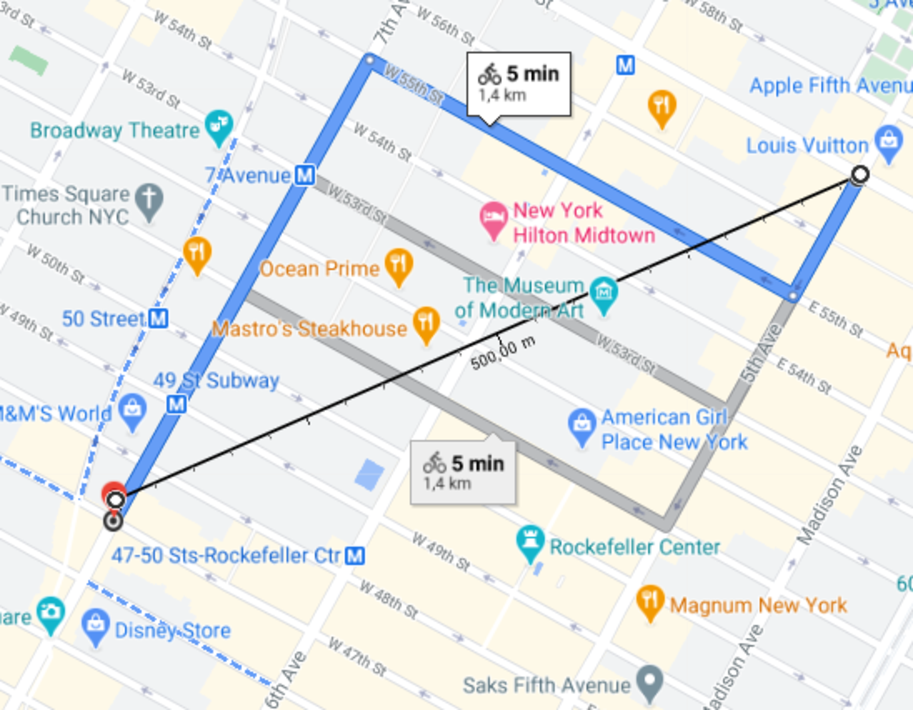
\includegraphics[width=\textwidth]{sources/max_manhattan/images/distance_manhattan2}
    \caption[Taxicab distance from times square to the trump tower]{Taxicab distance from times
    square to the Trump's tower. Notice that the black straight-line is depicting the Euclidean
    distance, and that the latter is shorter than the actual taxicab distance between  the two
    points.}
    \label{fig:max_manhattan:distance_manhattan}
\end{figure}

\section{Problem statement}
\begin{exercise}
\label{example:max_manhattan:exercice1}
Write a function that given \begin{enumerate*}
    \item a matrix $I$ of $n$ rows and $m$ columns and
    \item  an integer $K > 0$
\end{enumerate*}
returns a new matrix $M$ of size $n \times m$ where $M[i][j]$ contains the maximum value among the
elements in the Manhattan neighborhood of size $K$ for the cell $(i,j)$. The Manhattan neighborhood
of size $K$ for a cell $(i,j)$ is composed of all cell $(p,q)$ such that:
\begin{equation}
    N(i,j, K) = \{(p,q) | |i-p|+|j-q| \leq K\}
    \label{eq:max_manhattan:neighbood_equation}
\end{equation}


\end{exercise}
    %example1
    \begin{example}
        \label{example:max_manhattan:example1}
        \hfill \\
        Given: $I=
        \begin{bmatrix}
          1 & 2 & 3  \\
          4 & 5 & 6  \\
          7 & 8 & 9  
        \end{bmatrix}
      $
  and $K=1$ the function return $I=
  \begin{bmatrix}
      4 & 5 & 6  \\
      7 & 8 & 9  \\
      8 & 9 & 9  
    \end{bmatrix}
$
        
    \end{example}

    %example2
    \begin{example}
        \label{example:max_manhattan:example2}
        \hfill \\
        Given: $I=
        \begin{bmatrix}
          1 & 2 & 3  \\
          4 & 5 & 6  \\
          7 & 8 & 9  
        \end{bmatrix}
      $
  and $K=2$ the function return $I=
  \begin{bmatrix}
      7 & 8 & 9  \\
      8 & 9 & 9  \\
      9 & 9 & 9  
    \end{bmatrix}
$
        
    \end{example}




\section{Clarification Questions}

\begin{QandA}
    \item \begin{questionitem} \begin{question}   \end{question}      
    \begin{answered}
        \textit{}
    \end{answered} \end{questionitem}
    
\end{QandA}

\section{Discussion}
\label{max_manhattan:sec:discussion}

\subsection{Brute-force}
\label{max_manhattan:sec:bruteforce}
%You can optimize by only using N*M*2 space . see solution 2
This problem can be  tackled by using a brute-force approach that blindly calculates the answer for each cell as per the problem statement. 
All that is needed to find the answer for the cell $(i,j)$ is to calculate the maximum among the cells that are at a Manhattan distance of at most $K$ from it (the cells that are part of the Manhattan
neighborhood of size $K$). Therefore, the problem boils down to figuring out the neighborhood for a
given cell. Figure \ref{fig:max_manhattan:neighborhood} shows an example of such a neighborhood
where the numbers inside the cells represent the distance from the cell $(i,j)$ at the center. 
\begin{figure}
    \centering
    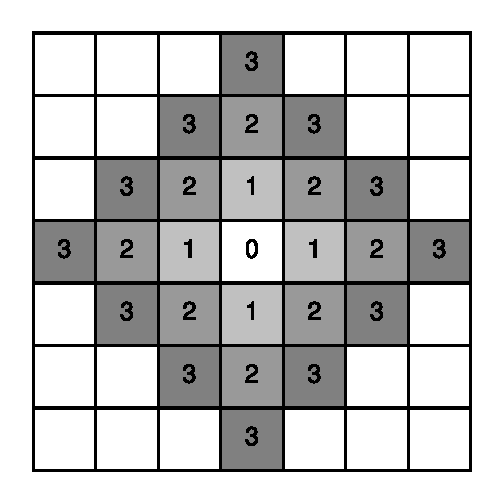
\includegraphics[width=\textwidth]{sources/max_manhattan/images/neighborhood}
    \caption[Cells in the Manhattan neighborhood of size $3$.]{Cells in the Manhattan neighborhood
    of size $3$. The numbers in each cell represent the Manhattan distance from the central cell.}
    \label{fig:max_manhattan:neighborhood}
\end{figure}
Given a cell $(i,j)$, figuring out exactly which cells are part of the neighborhood and which are
not is not particularly difficult. Instead of coming up with a way of
generating such a list of cells, it is easier to loop over all the cells within a square of size
$2K$ having cell $(i,j)$ at its center, and to ignore the ones that do not satisfy Equation
\ref{eq:max_manhattan:neighbood_equation}. Because both 
\begin{enumerate*}
    \item the number of cells in the neighborhood and 
    \item the number of cell in such square \end{enumerate*} is quadratic in $K$, then,
asymptotically speaking, the additional work required by visiting cells that are inside the area of
cells we are looping on but not part of the neighborhood does not really make any difference.
Listing \ref{list:max_manhattan:bruteforce} shows an implementation of this idea. This approach is
clearly correct and has a time complexity of $O(nmK^2)$ as for each of the $nm$ cells of the matrix
we do exactly $K^2$ work. The space complexity is $O(1)$ as no additional space is used other than
the second matrix we must return.
\lstinputlisting[language=c++, caption={Brute Force solution to the problem of finding the max cell within the manhattan neighborhood of size $K$.},label=list:max_manhattan:bruteforce]{sources/max_manhattan/max_manhattan_solution1.cpp}


\subsection{Dynamic Programming}
\label{max_manhattan:sec:DP}
As previously stated, the brute-force solution works by blindly finding the solution for each cell without taking into
consideration whether we can use the information already calculated for other cells.  Consider the matrix shown in Figure
\ref{fig:max_manhattan:neighborhoodDP1_1} showing the neighborhood of size $1$ for the cells 
\begin{itemize*}
    \item $(x,y)$ (center)
    \item $(x+1,y)$ (right)
    \item $(x-1,y)$ (left)
    \item $(x,y-1)$ (top)
    \item $(x,y+1)$ (down)
\end{itemize*}
and Figure \ref{fig:max_manhattan:neighborhoodDP1_2} showing the neighborhood of size $2$ for the
cell $(x,y)$. Note that the latter is composed by the union of the neighborhoods of size $1$ shown
in Figure \ref{fig:max_manhattan:neighborhoodDP1_1}. Therefore, if we know the answer for $K=1$ for
the cells 
\begin{itemize*}
    \item $(x,y)$
    \item $(x+1,y)$
    \item $(x-1,y)$
    \item $(x,y-1)$
    \item $(x,y+1)$ \end{itemize*} we can easily calculate the answer for $K=2$ for the cell $(x,y)$
without having to look at all the $12$ cells composing its Manhattan neighborhood of size $2$.



\begin{figure}
    \vspace*{-0.5in}
    %\hspace*{-0.5in}
    \centering
    
    \begin{subfigure}[t]{1.0\textwidth}
        \centering
        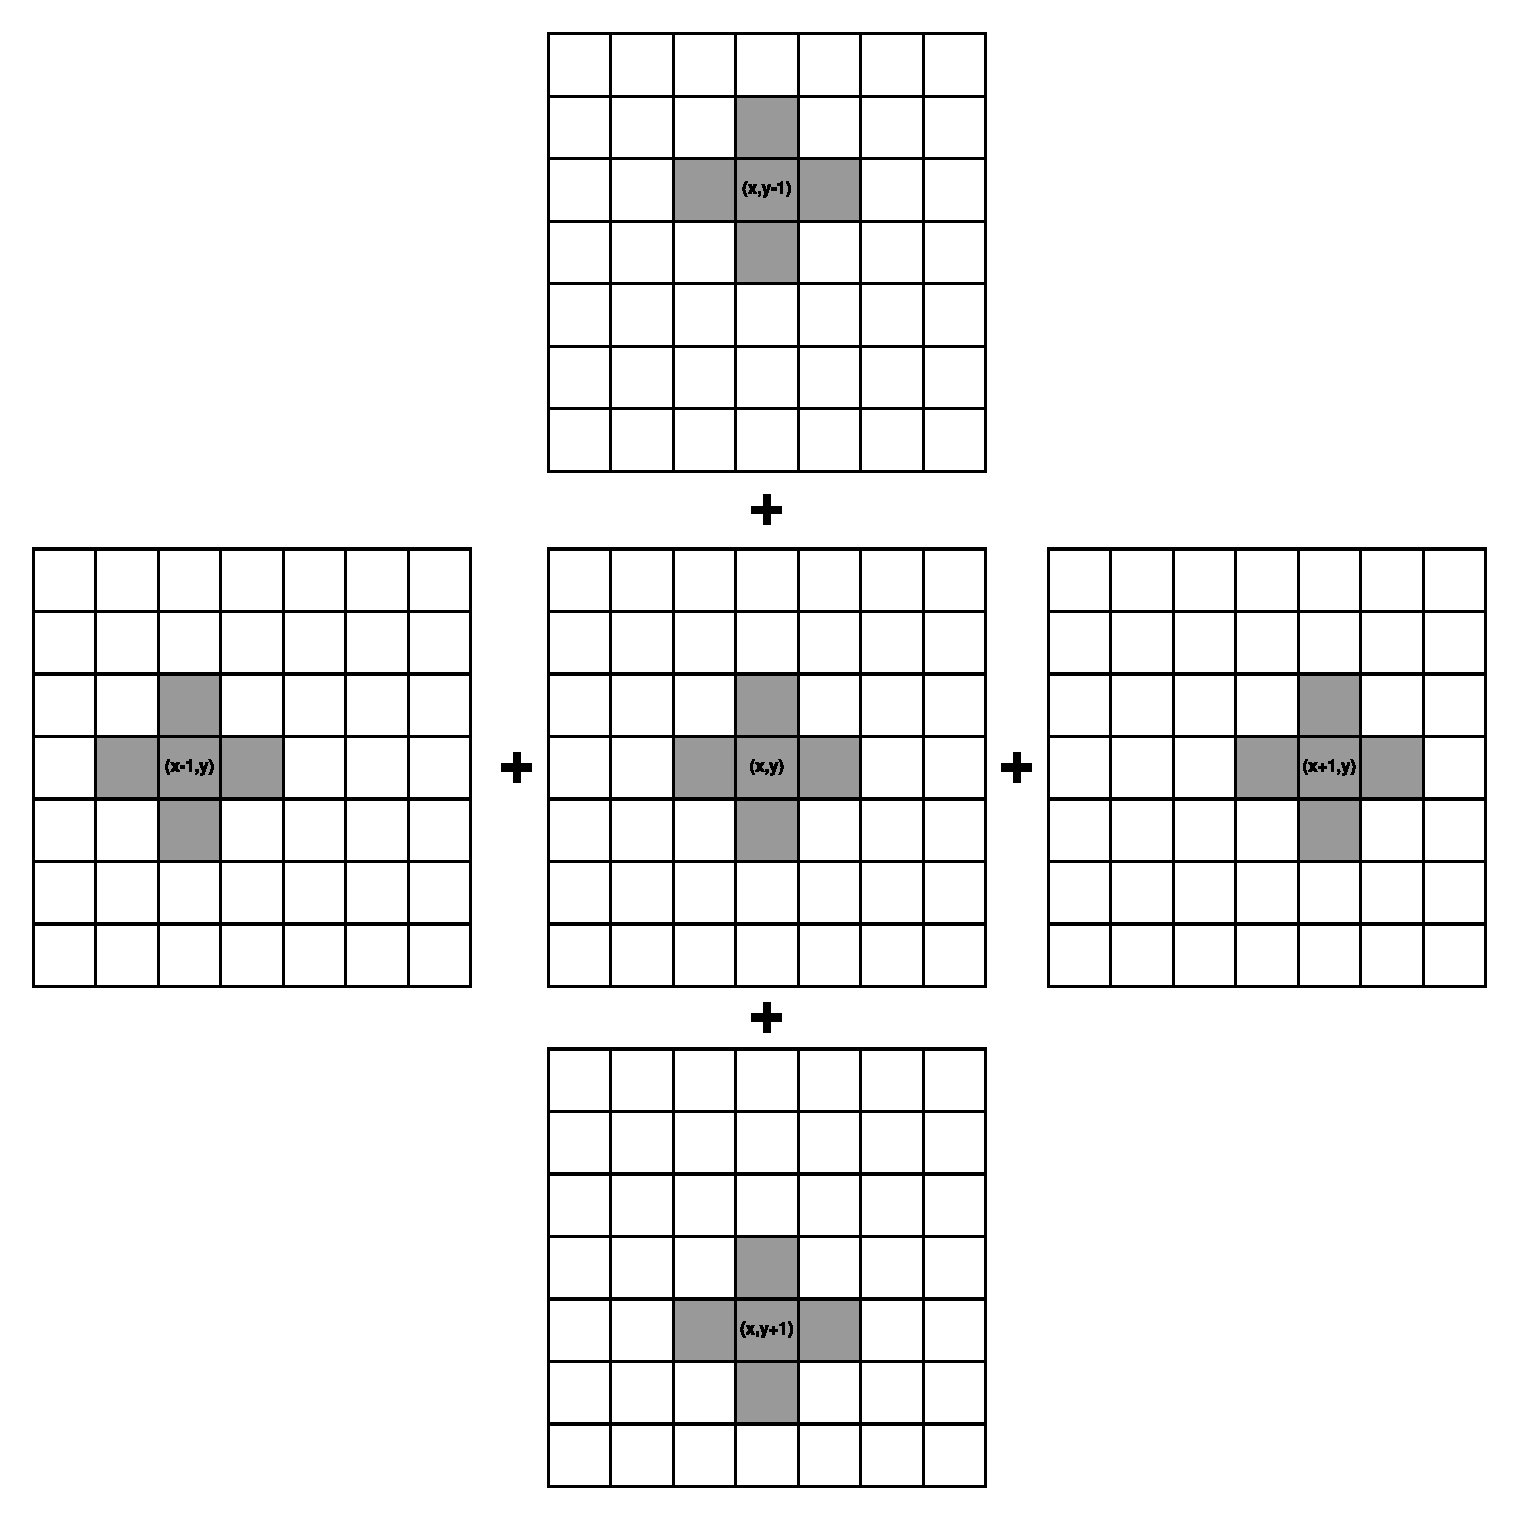
\includegraphics[width=\textwidth]{sources/max_manhattan/images/neighborhoodDP1_1}
        \caption[]{Manhattan neighborhoods of size $1$ for the cells:  $(x,y)$ (center), $(x+1,y)$ (right), $(x-1,y)$ (left), $(x,y-1)$ (top) and $(x,y+1)$ (down).}
        \label{fig:max_manhattan:neighborhoodDP1_1}
     \end{subfigure}
    
     \hfill
    
    \begin{subfigure}[t]{0.4\textwidth}
        \centering
        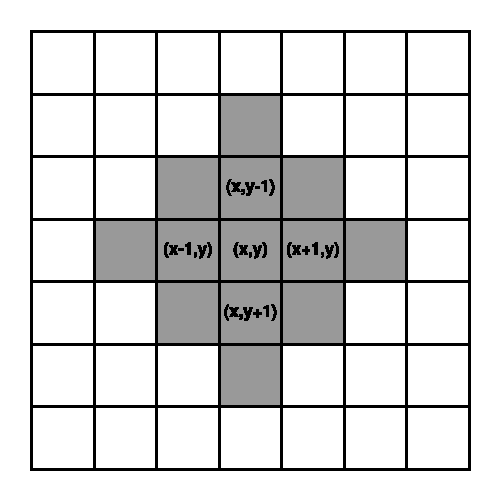
\includegraphics[width=\textwidth]{sources/max_manhattan/images/neighborhoodDP1_2}
        \caption[]{Neighborhood of size $2$ for the cell $(x,y)$ obtained by the union of the
        neighborhood depicted in Figure\ref{fig:max_manhattan:neighborhoodDP1_1}.}
        \label{fig:max_manhattan:neighborhoodDP1_2}
     \end{subfigure}
     \label{}
     \caption{}
\end{figure}

We can apply the same line of reasoning to find the answer for $K=3$. Figure
\ref{fig:max_manhattan:neighborhoodDPK2_1} shows  the neighborhoods of size $2$ for the cells 
\begin{itemize*}
    \item $(x,y)$
    \item $(x+1,y)$
    \item $(x-1,y)$
    \item $(x,y-1)$
    \item $(x,y+1)$ \end{itemize*} and and Figure \ref{fig:max_manhattan:neighborhoodDPK2_2} shows
the neighborhood of size $3$ for the cell $(x,y)$. Also in this case the latter can be obtained by
the union of all the cells in Figure \ref{fig:max_manhattan:neighborhoodDPK2_1} and therefore, if we
have the answer for all the sub-problems where $K=2$ we can obtain the answer for the sub-problems
where $K=3$ without having to scan the entirety of the neighborhood of size $3$ for $(x,y)$. We only
have to find the maximum among $5$ elements instead of having to look into $25$ cells. This idea can
be generalized and its formalization is shown in Equation \ref{eq:max_manhattan:dpformula}. The
formula is saying that we can obtain the answer for $K=0$  by simply returning the value of
the cell $(i,j)$. For $K>0$, we only have to return the max among the neighboring north,south, west
and east cells of $(i,j)$ for the same subproblem where $K-1$.

\hspace{-0.5in}
\vspace{-0.051in}
\begin{equation}
    \begin{cases}
        S(0,i,j) = I[i][j] \\
        S(K,i,j) = \max \Big [ S(K-1,i,j), S(K-1,i+1,j),\;S(K-1,i-1,j),\;S(K-1,i,j+1),\;S(K-1,i,j-1) \Big ] \\
     \end{cases}
    \label{eq:max_manhattan:dpformula}
\end{equation}

\begin{figure}
    \vspace*{-0.5in}
    %\hspace*{-0.5in}
    \centering
    
    \begin{subfigure}[t]{1.0\textwidth}
        \centering
        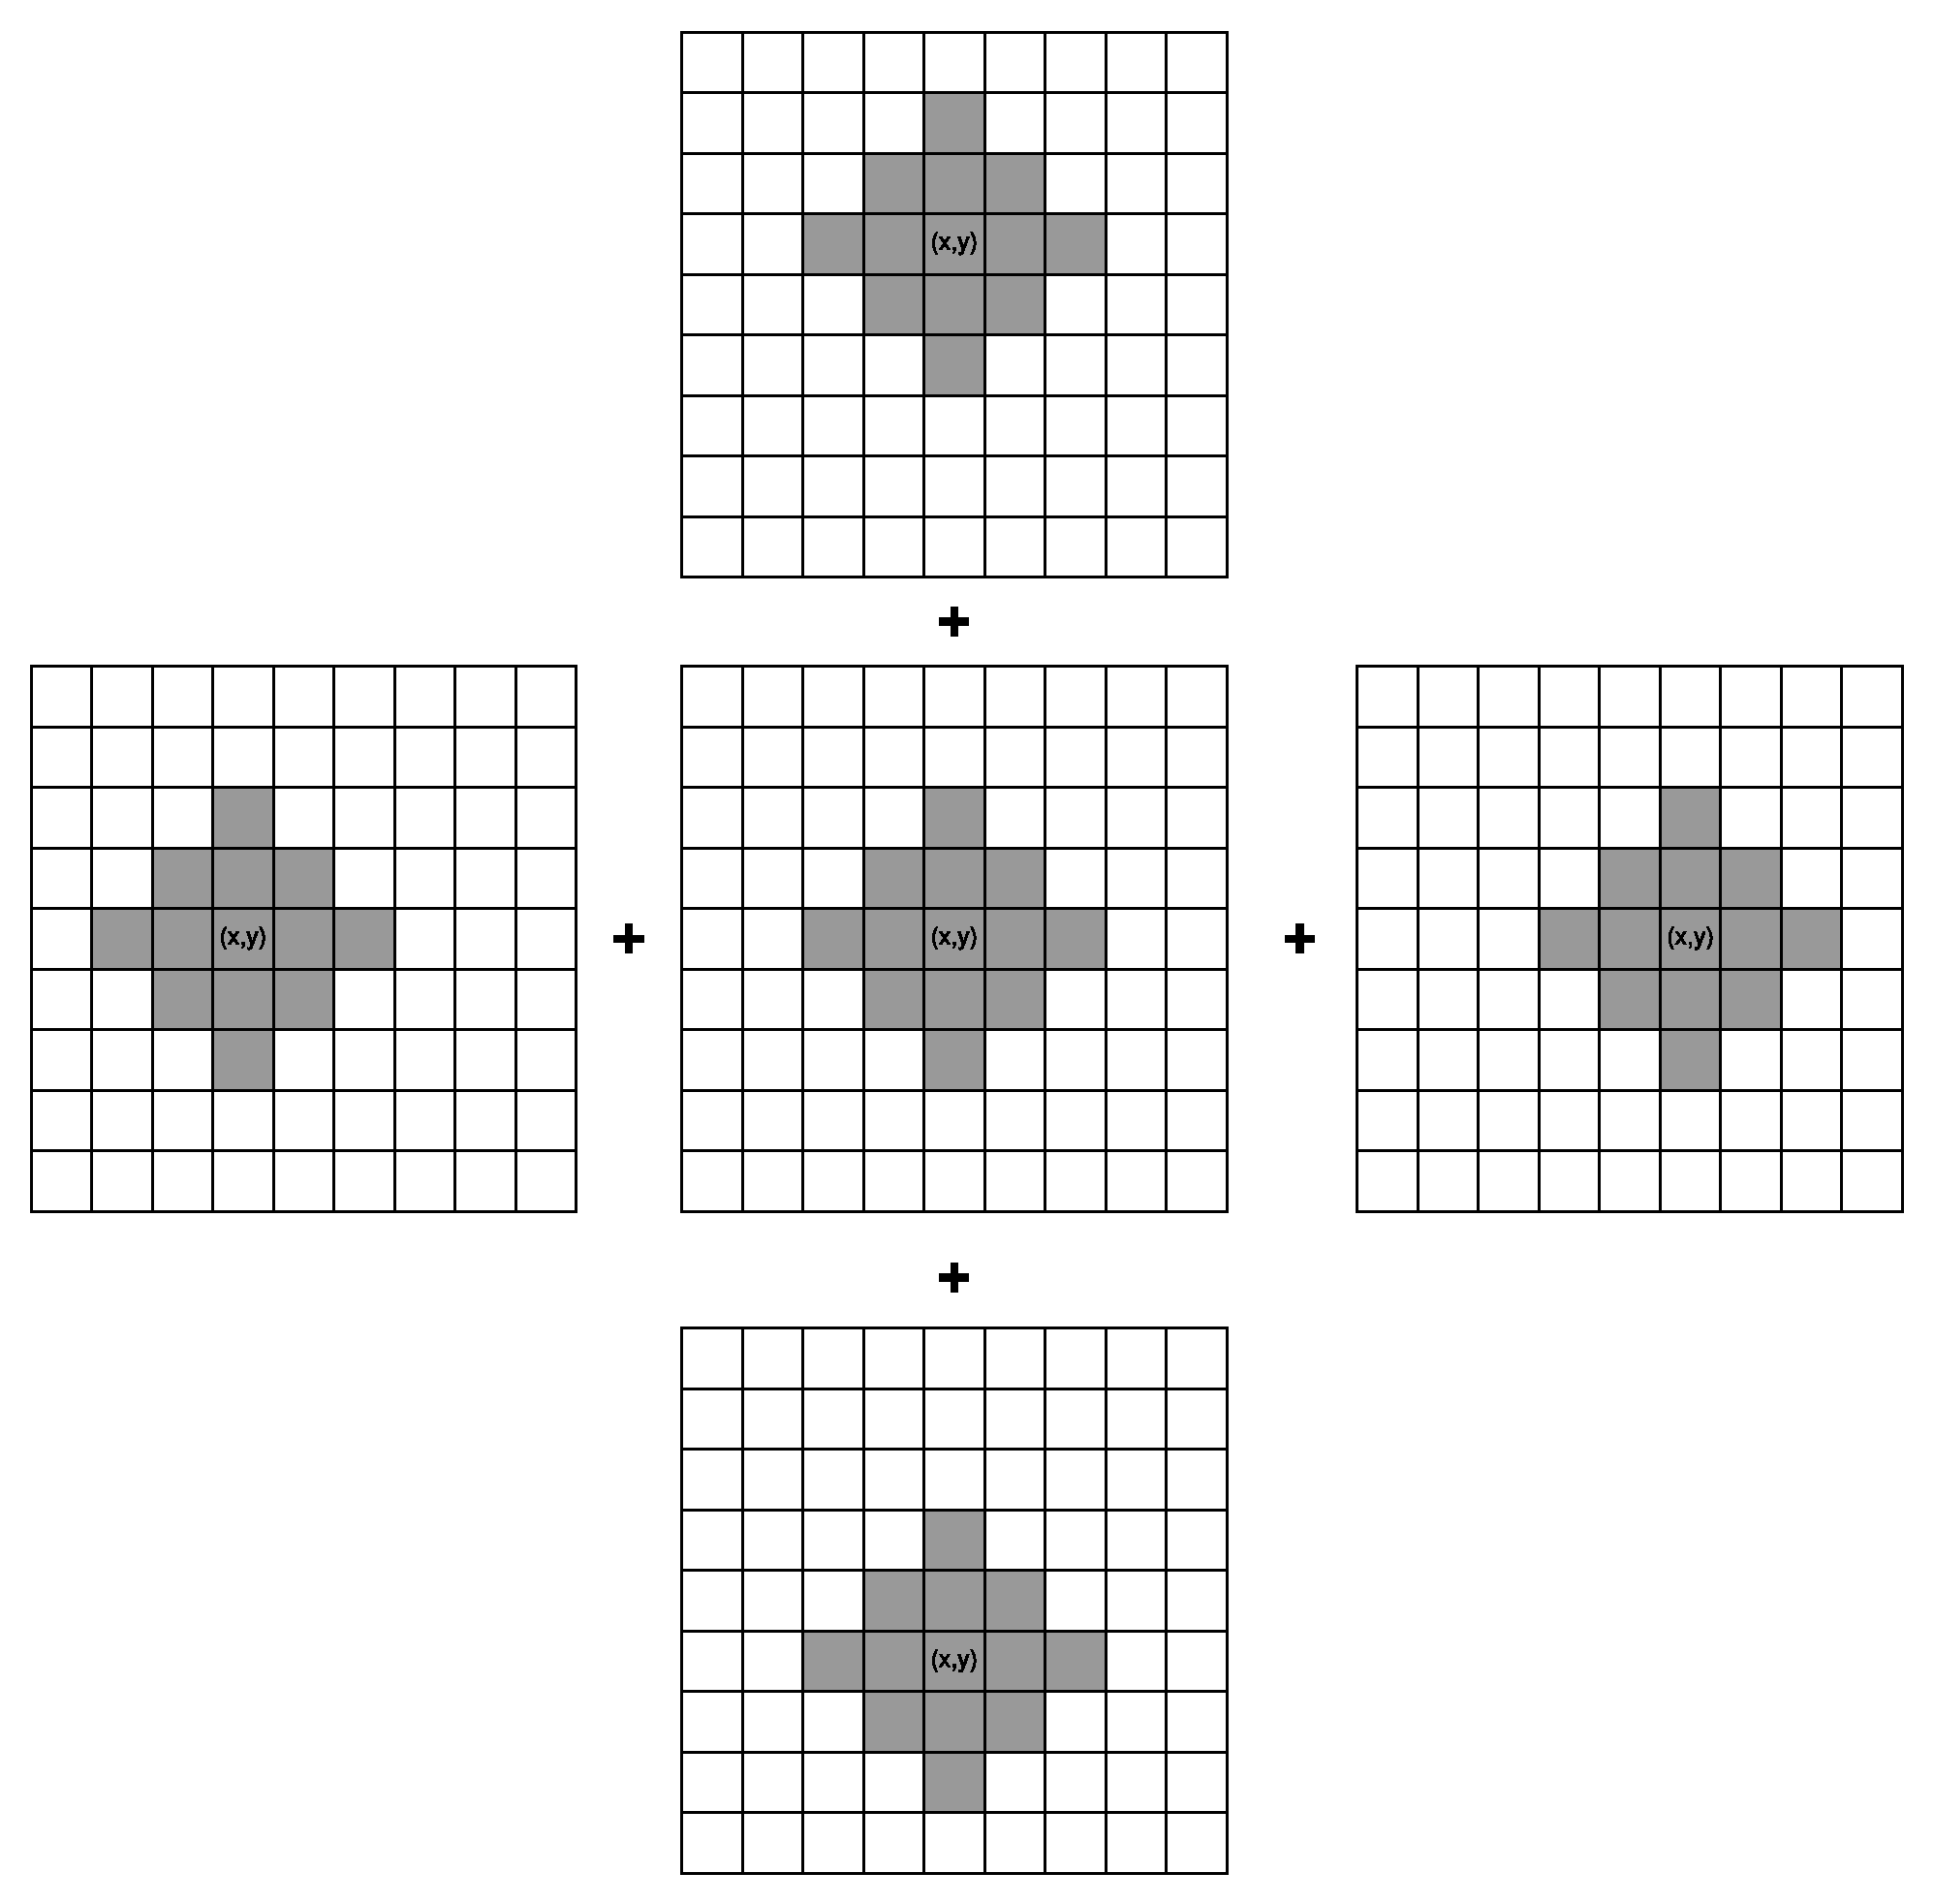
\includegraphics[width=\textwidth]{sources/max_manhattan/images/neighborhoodDPK2_1}
        \caption[]{Manhattan neighborhoods of size $1$ for the cells: $(x,y)$ (center), $(x+1,y)$ (right), $(x-1,y)$ (left), $(x,y-1)$ (top) and $(x,y+1)$ (down).}
        \label{fig:max_manhattan:neighborhoodDPK2_1}
    \end{subfigure}
    
    \hfill
    
    \begin{subfigure}[t]{0.4\textwidth}
        \centering
        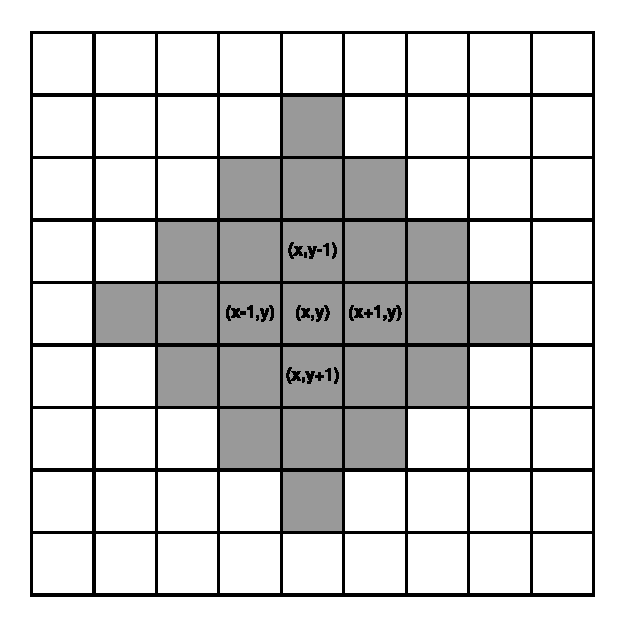
\includegraphics[width=\textwidth]{sources/max_manhattan/images/neighborhoodDPK2_2}
        \caption[]{Neighborhood of size $3$ for the cell $(x,y)$ obtained by the union of the
        neighborhood depicted in Figure\ref{fig:max_manhattan:neighborhoodDPK2_1}.}
        \label{fig:max_manhattan:neighborhoodDPK2_2}
     \end{subfigure}
     \label{}
     \caption{}
\end{figure}


As with all dynamic programming problems, we have two ways to write the solution:
\begin{enumerate}
    \item top-down, where we use memoization to avoid making duplicate work
    \item bottom-up, where we solve subproblems in an ordered manner from the simplest to the
    hardest.
\end{enumerate}

\subsubsection{Top-down}
\label{sec:max_manhattan:topdown}
The top-down approach is possibly the easiest to write as we can translate $S(K,i,j)$ (see Equation
\ref{eq:max_manhattan:dpformula}) into a C++ recursive function, and we can use memoization (in the
form of a cache of size $K\times n\times m$) to store intermediate values of $S$ and avoid duplicate
work. Listing \ref{list:max_manhattan:dp_topdown} shows an implementation of this approach where
such a cache is implemented via a hashmap, which maps the arguments of $S$, all triplets $(K,i,j)$,
to integers. Notice that the function \inline{hash\_combine} and the function \inline{TupleHash} are
the machinery that makes us use tuples of type \inline{std::tuple<int,int,int>} as keys in the Cache
(which has type \inline{std::unordered_map}). \inline{TupleHash} uses \inline{hash\_combine} to
calculate the hash value for a given \inline{std::tuple<int,int,int>}. The main driver function is
named \inline{max\_manhattan\_matrix\_k\_DP\_topdown} and the sole purpose is to create the
memoization cache and then to call the C++ equivalent of function $S$ (see Equation
\ref{eq:max_manhattan:dpformula}): \inline{max\_manhattan\_matrix\_k\_DP\_topdown\_helper}. The
latter is a recursive function that takes as input
\begin{enumerate*}
    \item the original input matrix $I$ (which is never modified and is only passed along as a
    reference),
    \item $K$, the max distance at which we search for the max value in $I$ ,
    \item \inline{cell}, which contains the coordinate of the cell for which we are finding an
    answer and finally
    \item the memoization cache where we store the answers for a given $K$ and \inline{cell}.
\end{enumerate*}

The first thing we do is to unpack the cell into two separate variables representing the row and the
column of a cell: $i,j$. If the coordinates of the cell are outside the boundaries of $I$ then there
is no answer for such a cell and we return the smallest possible int. Moreover if $K=0$, as per
Equation \ref{eq:max_manhattan:dpformula}, the answer is the value of the cell $(i,j)$ When we have
already calculated the solution to this problem (i.e. for the same values of $K,i,j$) then we
simply return the memoized value. In all  other cases we have to do the actual work and perform
the recursive calls to get the answer for the subproblems for the neighboring cells at the previous
value of $K$:
\begin{itemize}
    \item \inline{max\_manhattan\_matrix\_k\_DP\_topdown\_helper(K-1,i-1,j)}
    \item \inline{max\_manhattan\_matrix\_k\_DP\_topdown\_helper(K-1,i+1,j)}
    \item \inline{max\_manhattan\_matrix\_k\_DP\_topdown\_helper(K-1,i,j+1)}
    \item \inline{max\_manhattan\_matrix\_k\_DP\_topdown\_helper(K-1,i,j-1)} \end{itemize}.

The time and space complexity of this approach is $O(nmK)$. The proof is quite simple and it boils
down to the following facts:
\begin{enumerate}
    \item there are exactly $n\times m \times K$ different unique ways we can call the recursive
    function.
    \item each function call is memoized. This means that redundant work is avoided, therefore we do
    not do the work for a recursive call that has already been fully executed.
\end{enumerate}
Each entry in the memoization cache costs $4$ integers for a total of $O(nmK)$.

\lstinputlisting[language=c++, caption={DP top-down solution to the problem of finding the max cell within the manhattan neighborhood of size $K$.},label=list:max_manhattan:dp_topdown]{sources/max_manhattan/max_manhattan_solution2.cpp}



\subsubsection{Bottom-up}
If we pay closer attention to Equation \ref{eq:max_manhattan:dpformula} or, equivalently to the
top-down implementation in Listing \ref{list:max_manhattan:dp_topdown} we immediately notice that in
order to calculate all the values of $S(K,i,j)$ for a given $K$ we only need the values of $S$ for
$K-1$. Because we know the solution to the sub-problems where $K=0$, we can immediately solve
all the problems where $K=1$. At this point the values for the sub-problems where $K=0$ are not
needed anymore and we can throw them away and use that space to store the solution for the
sub-problems where $K=1$. Now that we have the solution for all sub-problems where $K=1$, we can proceed and calculate the
solutions for $K=2$. We apply the same line of reasoning to the rest of the sub-problems
 until we reach the value of $K$ we need.

The bottom-up approach is built on this idea and works by iteratively computing the answers for
sub-problems where $K-1$ before moving on to calculating the answer for the sub-problems for the next
value of $K$. This can be implemented by using two matrices of the same size of $I$:
\begin{itemize}
    \item $M_{K-1}$: storing the values of the sub-problems for the previous value of $K$ we are
    trying to compute during this step.
    \item $M_{K}$ which is the space where we write the answers for the sub-problems we calculate
    during this step.
\end{itemize}
When $M_{K}$ is full and ready, it can be copied into $M_{K-1}$ and continue to process the next
value of $K$. In other words, $M_{K}$ is a working space where the solutions to the sub-problems for
the current $K$ are stored, and $M_{K-1}$ contains all the answers for the sub-problems necessary to
calculate the answers at the step.

The computation of a value of $M_{K}$ uses the same idea as the top-down approach: the value of
to $M_K[i][j]$ is the maximum  among the following five values: 
\begin{enumerate*}
    \item $M_{K-1}[i][j]$
    \item $M_{K-1}[i+1][j]$
    \item $M_{K-1}[i-1][j]$
    \item $M_{K-1}[i][j+1]$
    \item $M_{K-1}[i][j-1]$
\end{enumerate*}

Note that at any time all the space we need is the space for storing the solution for the
sub-problems for two different values of $K$. This translates into a significant reduction in  space
complexity compared to the top-down approach described in Section \ref{sec:max_manhattan:topdown} which
is $O(nm)$ in this approach. 

Listing \ref{list:max_manhattan:dp_bottomup} shows an implementation of this idea. Note that in
the actual code $M_{K-1}$ and $M_{K}$ are the variables \inline{previous} and \inline{current},
respectively. 
\lstinputlisting[language=c++, caption={DP bottom-down solution to the problem of finding the max cell within the manhattan neighborhood of size $K$.},label=list:max_manhattan:dp_bottomup]{sources/max_manhattan/max_manhattan_solution3.cpp}

%This problem can be solved easily using dynamic programming. DP recurrence: dp[k][i][j] = ans. for
%kth manhattan distance for element (i,j) dp[k+1][i][j] = max(dp[k][i-1][j], dp[k][i+1][j],
%dp[k][i][j-1], dp[k][i][j+1], dp[k][i][j] ) Recurrence is easy to get once you draw the figure.

%%%%%%%%%%%%%%%%%%%%%%%%%%%%%%%%%%%%%%%%%%%%
%               Appendices
%%%%%%%%%%%%%%%%%%%%%%%%%%%%%%%%%%%%%%%%%%%%

\chapter{Appendices}
%% @Author: Davide Spataro
% @Date:   2020-10-25 
% @Last Modified by:   Davide Spataro
% https://www.topcoder.com/community/competitive-programming/tutorials/dynamic-programming-from-novice-to-advanced/
% file:///home/knotman/Downloads/DYNAMIC_PROGRAMMING_-_ITS_PRINCIPLES_APPLICATIONS_.pdf
% http://smo.sogang.ac.kr/doc/bellman.pdf 
\section*{Dynamic Programming}
\label{sect:appendix:DP}

Dynamic programming (DP) is a popular technique for solving a certain class of
optimization problems efficiently and is accredited to the American Scientist
Richard Bellman\cite{bellman1954}. He conied the term DP in the context of
solving problems involving a serie of best decision one after the other. 
The word \textit{programming} can be a bit deceiving for
computer scientist of programmers in general but it has really little to do with
computer programming and it is infact intended as a set of rules to 
follow to solve a certain problem and it is refeered specifically to the
solution to find an optimal military schedule for logistics (and has more or
less the same meaning as linear programming or linear optimization).  These rules can of course be coded and
executed by a computer but can be easily followed on paper for instance. 
Dynamic programming is better thought as an optimization approach rather than an
method or framework where a complex optimization problem is transformed into a sequence of
smaller (and simpler) problems. The very essence of DP is its multi-stage
optimization procedure. DP does not provide directly with the
instruction on how to solve a particular problem, but instead provides a general
framework that requires creativity and non trivial effort/insights so that a
problem formulation can be adapted and casted within the DP framework bounds.
This is possibly the reason why DP is considered a rather hard topic and it is
particularly feared during interviews. 

This chapter is not intended to be a full treatement of DP, and we will
introduce and describe it to the level that is necessary to understand and
better tackle DP interview problems. For a more comprenshive material on DP
please refer to \cite{bellman1954, cormen2009}.

The gist of the DP approach is that we aim at breaking down a problem into
simpler sub-problems recursively. If it is possible to do so, then the problem
at hand is said to have the \textbf{optimal substructure} property i.e. it can
be solved by using optimal solution to subproblems. But having the optimal
substructure property alone is not enough to prefer a DP approach to another
when trying to solve the same problem. This is because DP really shines when a
problem also exposes the \textbf{overlapping subproblems} property i.e. when the
subproblems are reused several times. A classic example if the
Fibonacci Sequence. In order to calculate $F(n)$ we need to solve two subproblems:
$F(n-1)$ and $F(n-2)$ and adding them up. But for solving $F(n-1)$ we need to
solve $F(n-2)$ \textbf{again}. The value for the subproblem $F(n-2)$ is thus
reused and this makes the Fibonacci problem exposed the optimal substructure
property. 
Dynamic programming takes care of this fact by making sure of solving each
subproblem only once. Usually this can be achieved into two ways:
\begin{description}
    \item [Top-down] This is usually the easiest of the two, by being a direct
    derivation from the recursive formulation of the problem. If the problem can
    be formulated recursively in terms of solution then solution to subproblems
    can be \textit{memoized}\footnote{From the latin word \textit{memorandum}
    which means to be remembered. It is basically a way of remembering the
    result of a function for a certain set of inputs call by storing it in a
    cache.} in a cache. 
    When a subproblem is reused then the
    (potentially expensive) recursive call is avoided and the cached result is
    returned instead. 
    \item [Bottom-up] We can try to reformulate the problem by twisting and
    massaging  the  recursive formulation so that the subproblems are solved
    first (thus effectively removing the recursion) and build the solution to
    the bigger problem from the bottom. This is usually done by working in a
    sort of tabular form where entries of the table for larger problems are
    filled by using  entries for solution to smaller problems that we have
    already solved. For instance, when solving the problem of finding the
    $10^{th}$ Fibonacci number $F(10)$, we can start from the known values for
    $F(0)$ and $F(1)$ and working our way up to $F(2)$  by using $F(1)$ and
    $F(2)$. Once F(2) is ready we can move up to F(3), and so on when we have
    the values for $F(8)$ and $F(9)$ we proceed with calculating $F(10)$.
\end{description}

DP has found application in many field of science such as Control theory,
Bioinformatics AI and operations research. There are a number of problems in
computer science that can be solved by using DP such as the 
\begin{itemize}
    \item Longest Common (or increasing) Subsequence
    \item Weighted Interval Scheduling
    \item Chain Matrix Multiplication
    \item Subset sub
    \item String edit distance
    \item Coin change
    \item 0/1 knapsack problem
    \item Graph shortest path
\end{itemize}

In the next section we will shortly review a number of DP problem focusing on
the key ideas that allow a problem to be approached and solved  using DP.

\subsection*{Fibonacci Sequence}
Computing the $n^{th}$ number of the Fibonacci sequence is probably one of the
most common introductionary example of DP. The Fibonacci sequence recursive
formulation is ready to be solved using a top-down DP approach. Listing
\ref{list:app:dp:canonical} shows a C++ function that calculated the $n^{th}$ Fibonacci
number.
\lstinputlisting[language=c++, caption={Canonical recursive C++ implementation of a function returning the $n^{th}$ Fibonacci number.},label=list:app:dp:canonical]{/home/dspataro/git/algorithm_articles/sources/appendices/fibonacci_canonical.cpp}
Notice that for instance when $F(6)$ a call tree is produced where the same call
is repeated more than once as shown in the list below. $F(2)$ has been
calculated $5$ times!
\begin{itemize}
    \item $F(6) = F(5)+F(4)$
    \item $F(6) = (F(4)+F(3)) + (F(3)+F(2))$
    \item $F(6) = ((F(3)+F(2))+(F(2)+F(1))) + ((F(2)+F(1))+(F(1)+F(0)))$
    \item $F(6) = (((F(2)+F(1))+(F(1)+F(0)))+((F(1)+F(0))+F(1))) + (((F(1)+F(0))+F(1))+(F(1)+F(0)))$
    \item $F(6) = ((((F(1)+F(0))+F(1))+(F(1)+F(0)))+((F(1)+F(0))+F(1))) + (((F(1)+F(0))+F(1))+(F(1)+F(0)))$
\end{itemize}

Listing \ref{list:app:dp:fib} can be improved dramatically if we memoize the function calls
that have been already calculated. This way no duplicate work is done. W.r.t the
previous example, from the second time the value of $F(2)$ is needed, no
additional work is done, as the value in the cache is returned.
\lstinputlisting[language=c++, caption={Canonical recursive top-down Dynamic Programming C++ implementation of a function returning the $n^{th}$ Fibonacci number.},label=list:app:dp:fib]{/home/dspataro/git/algorithm_articles/sources/appendices/fibonacci_dp_top_down.cpp}

%\section{Prefix sum}
\label{sect:appendix:prefix_sum}
In computer science, the prefix sum, cumulative sum, inclusive scan, or simply scan of a sequence of numbers x0, x1, x2, ... is a second sequence of numbers y0, y1, y2, ..., the sums of prefixes (running totals) of the input sequence:
%% @Author: Davide Spataro
% @Date:   2020-03-30 17:18:14
% @Last Modified by:   Davide Spataro
% @Last Modified time: 2020-03-30 17:28:08
\section{Binary Search}
\label{sect:appendix:binary_search}
\lipsum{1}
%%%%%%%%%%%%%%%%%%%%%%%%%%%%%%%%%%%%%%%%%%%%
%               BIBLIOGRAPHY
%%%%%%%%%%%%%%%%%%%%%%%%%%%%%%%%%%%%%%%%%%%%

%
%from documentation
%\newacronym[⟨key-val list⟩]{⟨label ⟩}{⟨abbrv ⟩}{⟨long⟩}
%above is short version of this
% \newglossaryentry{⟨label ⟩}{type=\acronymtype,
% name={⟨abbrv ⟩},
% description={⟨long⟩},
% text={⟨abbrv ⟩},
% first={⟨long⟩ (⟨abbrv ⟩)},
% plural={⟨abbrv ⟩\glspluralsuffix},
% firstplural={⟨long⟩\glspluralsuffix\space (⟨abbrv ⟩\glspluralsuffix)},
% ⟨key-val list⟩}

\newacronym{cd}{CD}{compact disk}
\newacronym{utc}{UTC}{Coordinated Universal Time}
%\newacronym{adt}{ADT}{Atlantic Daylight Time}
%\newacronym{est}{EST}{Eastern Standard Time}
 
% Use the acronyms
\gls{utc} is 3 hours behind \gls{adt} and 10 hours ahead of \gls{est}.



%\addcontentsline{toc}{chapter}{\textcolor{ocre}{Glossary}}
%\printglossaries


%Print the glossary

\addcontentsline{toc}{chapter}{\textcolor{ocre}{Bibliography}}
%\chapter*{Bibliography}
%Print the glossary
\printbibliography	
	
%%%%%%%%%%%%%%%%%%%%%%%%%%%%%%%%%%%%%%%%%%%%
%               INDEX
%%%%%%%%%%%%%%%%%%%%%%%%%%%%%%%%%%%%%%%%%%%%	
	\cleardoublepage
	\phantomsection
	\setlength{\columnsep}{0.75cm}
	\addcontentsline{toc}{chapter}{\textcolor{ocre}{Index}}
	\printindex


	%\backmatter

\end{document}
